\section{Implementation and results}
\label{sec.results}

In this work the experiments used the OpenGL indirectly using the OpenSceneGraph~\cite{Burns2004}, a higher level, open-source, visualization framework. OpenSceneGraph provides a layer of abstraction over OpenGL in order to create the scene with memory managed objects, organized in a graph that provides the dependencies of each object and optimises the memory utilization and rendering speed. Although the high-level of abstraction, OpenSceneGraph provides mechanisms to create custom operations if needed. The main advantage of using OpenSceneGraph for fish tank visualization is the easy abstraction with the windowing system, which is abstracted using object modeling strategy, and the multiple displays infrastructure.

The FTVR has an extended field of view (FOV) of $120^{\circ}$ between the displays, as illustrated in Figure~\ref{fig.tv_setup}b. A large FOV has been reported as an important aspect of immersion of in VR systems~\cite{Hounsell2013}. The scene is projected using HCP combined with the stereo technique presented in Section~\ref{sec.holographic_emulation}. The position of the viewer is tracked by a Microsoft Kinect Sensor. The view frustum has with a range of 4 meters, $43^{\circ}$ vertical by $57^{\circ}$ horizontal field of view, and vertical tilt range of $\pm 27^{\circ}$. The sensor has an RGB camera that stores three channel data in a 1280x960 resolution, and an infrared (IR) emitter and an IR depth sensor. The emitter emits infrared light beams and the depth sensor reads the IR beams reflected back to the sensor. The reflected beams are converted into depth information measuring the distance between an object and the sensor. 

%In order to create the hologram, the concave volume formed by the tilt of the displays form the FTVR where VOI the emulated hologram is projected . The Figure~\ref{fig.tv_setup} show the setup of the experiment, with 2 stereo displays and the Kinect sensor. The area of tracking is shown by the frustum coming from the sensor. The tracking area can be easily extended with extra hardware. A previous setup had 2 kinect sensors placed on the base of each display to cover a larger area, but due hardware constrains, the setup has been reduced to only on sensor.

The implementation of the experiment used a face tracking library available in the Kinect SDK from Microsoft~\cite{Zhang2012}, which can track faces without prior training. The software can adjust the pitch angle of the sensor while it keeps the face in the center of the image. Ir order to remove the noise, the tracked movement is filtered by a step function in Equation~\ref{eq.step}; that takes displacements $x$ greater than 1 cm or the average of the displacements $\mu_x$ if smaller. Figure~\ref{fig.tracking} shows, on the right side, the video used in the face tracking and an overlay of a mask projected on of the video with the distance tracked. The position of the viewer is estimated by the position of the face.

\begin{equation}
  u(x)=\begin{cases}
    x, & \text{if $x>1$}.\\
    \mu_{x}, & \text{otherwise}.
  \end{cases}
  \label{eq.step}
\end{equation}

\begin{figure}[!hbt]
\centering
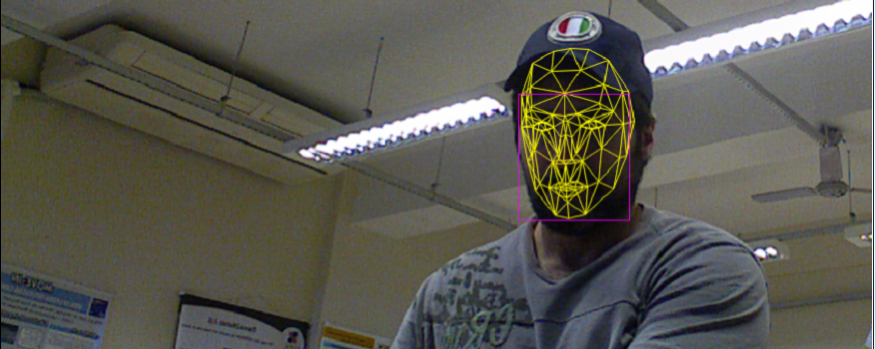
\includegraphics[width=0.7\linewidth,keepaspectratio=true]{figs/tracking_face.png}
\caption{Face tracking used to estimate the position of the viewer.}
\label{fig.tracking}
\end{figure}

The stereo rendering uses the horizontal half of each screen for each eye as shown in Figure~\ref{fig.split_screens}. The projection is displaced by a horizontal offset on each screen view (small arrows) in projection transform of Figure~\ref{fig.osg_pipeline}. The width of bezel of the displays is taken into account in the offset to preserve an hidden continuity between the displays. The tilt of the screens is placed in the view transform of the slave cameras.

The implementation emulated an hologram using the procedure described in Section~\ref{sec.holographic_emulation}, with objects centered in the origin of the scene, $M_{view}$, in order to produce the correct viewpoint and binocular parallax. The experiments with the holographic projection for off-centered objects are left for future work and out of the scope of this work.

